% Study overview (vector, TikZ), council round 31.10.2026 (brief 12, section 6.1).
% Copied from paper/figures/overview/fig_study_overview.tex (left untouched) and rebuilt:
%   (a) models: the R32 / V-scr seed pair and the architecture-by-initialization cells,
%   (b) fixed panels: CIFAR-10, CIFAR-100, ImageNetV2 (with same-recipe pairs),
%   (c) measurement: transfer matrix -> w, tau-bar, r -> sigma, rho, omega,
%   (d) registered test families and the conditioning-protocol layer.
% Carries no result numbers. The only numerals are model and run counts, read as macros from
% fig_study_overview_sayilar.tex, which fig_study_overview_veri.py writes from the frozen cell
% tables and checks against results/C1_REFERANS_FOYU.md.
% Build: bash paper/figures/konsey/fig_study_overview_derle.sh
\documentclass[border=3pt]{standalone}
\usepackage[T1]{fontenc}
% helvet italic TFMs are missing in this installation (phvro8t); Latin Modern sans is used.
\IfFileExists{lmodern.sty}{\usepackage{lmodern}}{}
\renewcommand{\familydefault}{\sfdefault}
\usepackage{amsmath,amssymb}
\usepackage{tikz}
\usetikzlibrary{positioning,fit,arrows.meta,calc,backgrounds}
% Generated by paper/figures/konsey/fig_study_overview_veri.py; do not edit by hand.
% Every count is read from the cell tables / Mantel files and checked against results/C1_REFERANS_FOYU.md.
\newcommand{\NmodCten}{20}
\newcommand{\NmodChun}{15}
\newcommand{\NmodIN}{14}
\newcommand{\SeedRtt}{3}
\newcommand{\SeedVscr}{3}
\newcommand{\SeedVin}{2}
\newcommand{\SeedRscr}{2}
\newcommand{\SeedRin}{2}
\newcommand{\PanelCten}{7}
\newcommand{\SecCten}{1}
\newcommand{\SeedChunR}{3}
\newcommand{\SeedChunV}{3}
\newcommand{\PanelChun}{7}
\newcommand{\SecChun}{2}
\newcommand{\PanelIN}{6}
\newcommand{\SecIN}{1}
\newcommand{\PairsIN}{3}
\newcommand{\TransIN}{4}
\newcommand{\UnpairedIN}{1}


% Okabe-Ito, same semantic assignment as the matplotlib council figures (konsey_ortak.py)
\definecolor{vit}{HTML}{D55E00}
\definecolor{rtf}{HTML}{0072B2}
\definecolor{rtt}{HTML}{56B4E9}
\definecolor{sym}{HTML}{009E73}
\definecolor{dir}{HTML}{E69F00}
\definecolor{pnl}{HTML}{999999}
\definecolor{ink}{HTML}{262626}
\definecolor{mute}{HTML}{6E6E6E}
\definecolor{pane}{HTML}{F6F7F9}
\hyphenpenalty=10000 \exhyphenpenalty=10000

\begin{document}
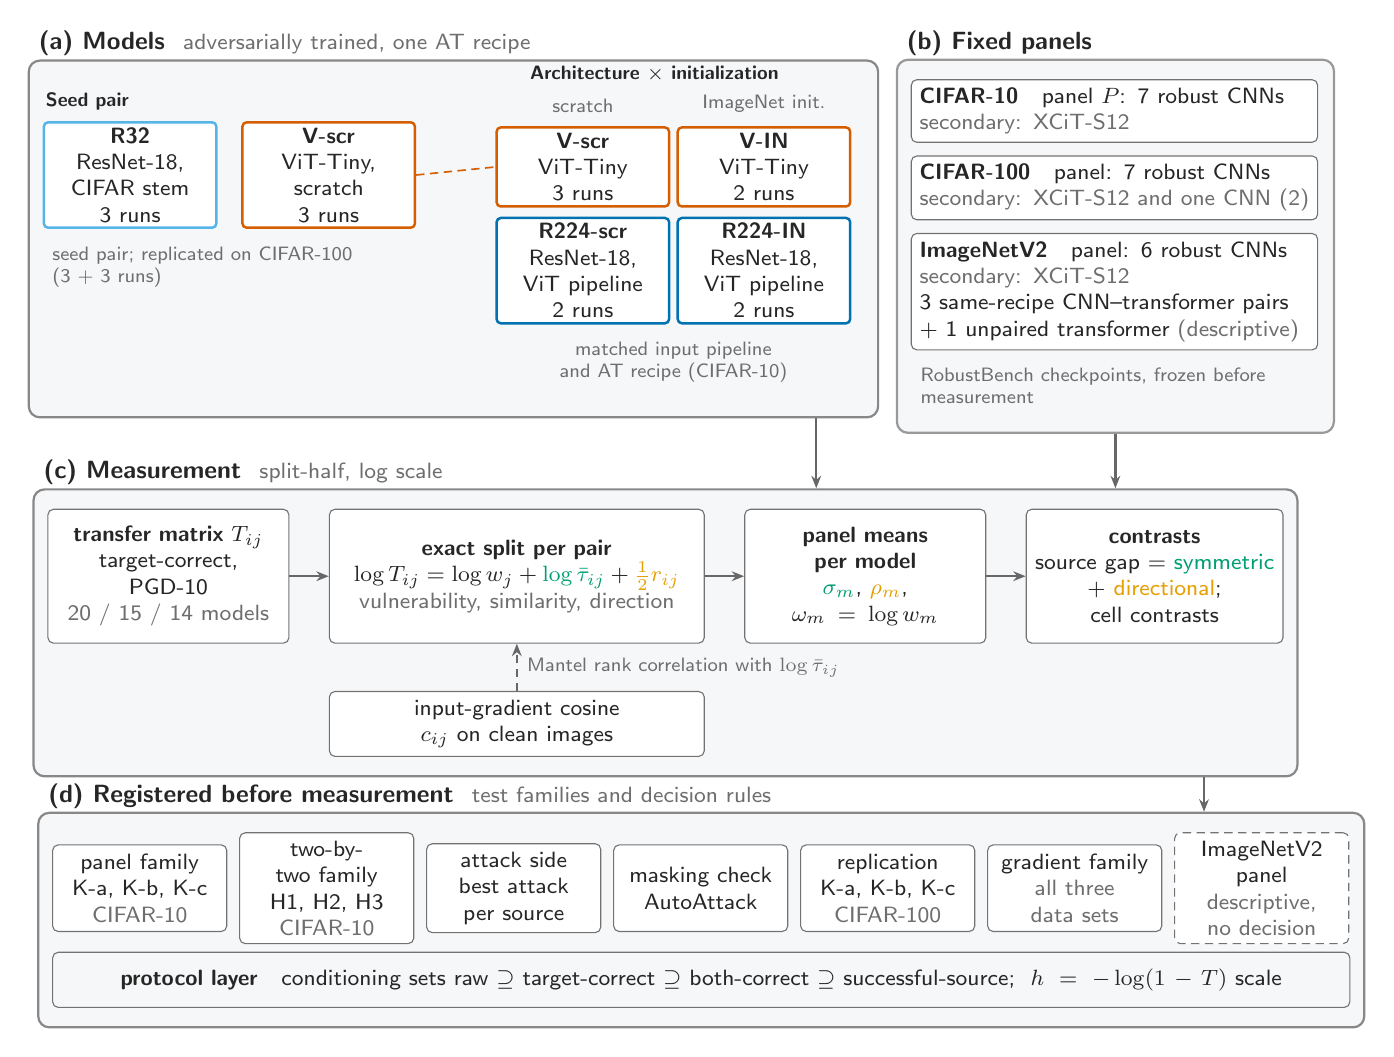
\begin{tikzpicture}[
  font=\footnotesize, text=ink,
  >={Stealth[length=4.5pt,width=3.5pt]},
  every node/.style={align=center},
  blk/.style={draw=ink!65, fill=white, rounded corners=2pt, inner sep=3pt, text width=#1},
  cell/.style={draw=#1, line width=0.9pt, fill=white, rounded corners=1.5pt, inner sep=2pt,
               text width=2.05cm, minimum height=9.5mm},
  fam/.style={blk=2.0cm, minimum height=11mm},
  cont/.style={draw=#1, line width=0.8pt, rounded corners=4pt, inner sep=5pt, fill=pane},
  arr/.style={->, line width=0.8pt, draw=ink!70},
  ttl/.style={font=\small\bfseries, text=ink, inner sep=1pt, anchor=south west},
  sub/.style={font=\scriptsize, text=mute},
]

% =============================================================== (a) MODELS =====
\node[cell=rtt] (r32) at (0.0, 0) {\textbf{R32}\\ResNet-18, CIFAR stem\\\SeedRtt\ runs};
\node[cell=vit, right=3mm of r32] (vp) {\textbf{V-scr}\\ViT-Tiny, scratch\\\SeedVscr\ runs};
\node[sub, anchor=north west, text width=4.6cm, align=left] (pairnote) at ($(r32.south west)+(0,-1mm)$)
  {seed pair; replicated on CIFAR-100\\(\SeedChunR\ + \SeedChunV\ runs)};
\node[font=\scriptsize\bfseries, anchor=south west, inner sep=1pt] at ($(r32.north west)+(0,1mm)$) {Seed pair};

% architecture-by-initialization cells
\coordinate (g0) at (5.75, 0.62);
\node[font=\scriptsize, text=mute, anchor=south] (hs) at ($(g0)+(0,0.05)$) {scratch};
\node[font=\scriptsize, text=mute, anchor=south] (hi) at ($(g0)+(2.30,0.05)$) {ImageNet init.};
\node[cell=vit, anchor=north] (cvs) at (g0) {\textbf{V-scr}\\ViT-Tiny\\\SeedVscr\ runs};
\node[cell=vit, anchor=north] (cvi) at ($(g0)+(2.30,0)$) {\textbf{V-IN}\\ViT-Tiny\\\SeedVin\ runs};
\node[cell=rtf, anchor=north] (crs) at ($(g0)+(0,-1.15)$) {\textbf{R224-scr}\\ResNet-18, ViT pipeline\\\SeedRscr\ runs};
\node[cell=rtf, anchor=north] (cri) at ($(g0)+(2.30,-1.15)$) {\textbf{R224-IN}\\ResNet-18, ViT pipeline\\\SeedRin\ runs};
\node[font=\scriptsize\bfseries, anchor=south west, inner sep=1pt] at ($(hs.north west)+(-0.2,0.05)$)
  {Architecture $\times$ initialization};
\node[sub, anchor=north, text width=4.6cm] (cellnote) at ($(crs.south)!0.5!(cri.south)+(0,-1mm)$)
  {matched input pipeline and AT recipe (CIFAR-10)};
\draw[densely dashed, draw=vit, line width=0.6pt] (vp.east) -- (cvs.west);

\begin{scope}[on background layer]
  \node[cont=ink!55, fit=(r32)(vp)(pairnote)(cvs)(cvi)(crs)(cri)(cellnote)(hs)(hi), inner ysep=9pt] (abox) {};
\end{scope}
\node[ttl] at ($(abox.north west)+(1mm,0)$) {(a) Models \ {\normalfont\footnotesize\color{mute}adversarially trained, one AT recipe}};

% =============================================================== (b) PANELS =====
\node[blk=4.95cm, align=left, anchor=north west] (pc10) at ($(abox.north east)+(4mm,-2.5mm)$)
  {\textbf{CIFAR-10}\quad panel $P$: \PanelCten\ robust CNNs\\{\color{mute}secondary: XCiT-S12}};
\node[blk=4.95cm, align=left, below=1.6mm of pc10] (pc100)
  {\textbf{CIFAR-100}\quad panel: \PanelChun\ robust CNNs\\{\color{mute}secondary: XCiT-S12 and one CNN (\SecChun)}};
\node[blk=4.95cm, align=left, below=1.6mm of pc100] (pin)
  {\textbf{ImageNetV2}\quad panel: \PanelIN\ robust CNNs\\{\color{mute}secondary: XCiT-S12}\\
   \PairsIN\ same-recipe CNN--transformer pairs\\+ \UnpairedIN\ unpaired transformer {\color{mute}(descriptive)}};
\node[sub, anchor=north west, text width=4.95cm, align=left] (pnote) at ($(pin.south west)+(0,-1mm)$)
  {RobustBench checkpoints, frozen before measurement};
\begin{scope}[on background layer]
  \node[cont=pnl, fit=(pc10)(pc100)(pin)(pnote), inner ysep=7pt] (bbox) {};
\end{scope}
\node[ttl] at ($(bbox.north west)+(1mm,0)$) {(b) Fixed panels};

% ========================================================== (c) MEASUREMENT =====
\coordinate (crow) at ($(abox.south west |- bbox.south)+(0,-0.95)$);
\node[blk=2.85cm, anchor=north west, minimum height=17mm] (m1) at ($(crow)+(0.25,0)$)
  {\textbf{transfer matrix} $T_{ij}$\\target-correct, PGD-10\\{\color{mute}\NmodCten\ / \NmodChun\ / \NmodIN\ models}};
\node[blk=4.55cm, right=5mm of m1, minimum height=17mm] (m2)
  {\textbf{exact split per pair}\\\mbox{$\log T_{ij}=\log w_j+{\color{sym}\log\bar\tau_{ij}}+{\color{dir}\tfrac12 r_{ij}}$}\\
   {\color{mute}vulnerability, similarity, direction}};
\node[blk=2.85cm, right=5mm of m2, minimum height=17mm] (m3)
  {\textbf{panel means per model}\\${\color{sym}\sigma_m}$, ${\color{dir}\rho_m}$, $\omega_m=\log w_m$};
\node[blk=3.05cm, right=5mm of m3, minimum height=17mm] (m4)
  {\textbf{contrasts}\\source gap $=$ {\color{sym}symmetric}\\$+$ {\color{dir}directional}; cell contrasts};
\node[blk=4.55cm, below=6mm of m2, minimum height=7mm] (g1)
  {input-gradient cosine $c_{ij}$ on clean images};
\draw[arr] (m1) -- (m2);
\draw[arr] (m2) -- (m3);
\draw[arr] (m3) -- (m4);
\draw[arr, densely dashed] (g1.north) -- node[right, font=\scriptsize, text=mute] {Mantel rank correlation with $\log\bar\tau_{ij}$} (m2.south);
\begin{scope}[on background layer]
  \node[cont=ink!55, fit=(m1)(m2)(m3)(m4)(g1), inner ysep=7pt] (cbox) {};
\end{scope}
\node[ttl] at ($(cbox.north west)+(1mm,0)$) {(c) Measurement \ {\normalfont\footnotesize\color{mute}split-half, log scale}};
\coordinate (aout) at ($(abox.south east)+(-8mm,0)$);
\draw[arr] (aout) -- (aout |- cbox.north);
\draw[arr] (bbox.south) -- (bbox.south |- cbox.north);

% ========================================================= (d) FAMILIES =====
\coordinate (drow) at ($(cbox.south west)+(0.25,-0.85)$);
\node[fam, anchor=north west] (f1) at (drow) {panel family\\K-a, K-b, K-c\\{\color{mute}CIFAR-10}};
\node[fam, right=1.5mm of f1] (f2) {two-by-two family\\H1, H2, H3\\{\color{mute}CIFAR-10}};
\node[fam, right=1.5mm of f2] (f3) {attack side\\best attack per source};
\node[fam, right=1.5mm of f3] (f4) {masking check\\AutoAttack};
\node[fam, right=1.5mm of f4] (f5) {replication\\K-a, K-b, K-c\\{\color{mute}CIFAR-100}};
\node[fam, right=1.5mm of f5] (f6) {gradient family\\{\color{mute}all three data sets}};
\node[fam, right=1.5mm of f6, densely dashed] (f7) {ImageNetV2 panel\\{\color{mute}descriptive,\\no decision}};
\path let \p1 = (f1.west), \p2 = (f7.east) in
  node[blk={\x2-\x1-6pt}, anchor=north west, fill=pane, minimum height=7mm] (prot) at ($(f1.south west)+(0,-2.5mm)$)
  {\textbf{protocol layer}\quad conditioning sets raw $\supseteq$ target-correct $\supseteq$ both-correct $\supseteq$ successful-source;
   \ $h=-\log(1-T)$ scale};
\begin{scope}[on background layer]
  \node[cont=ink!55, fit=(f1)(f7)(prot), inner ysep=7pt] (dbox) {};
\end{scope}
\node[ttl] at ($(dbox.north west)+(1mm,0)$) {(d) Registered before measurement \ {\normalfont\footnotesize\color{mute}test families and decision rules}};
\coordinate (cout) at ($(cbox.south east)+(-12mm,0)$);
\draw[arr] (cout) -- (cout |- dbox.north);

\end{tikzpicture}
\end{document}
